% Main-manuscript figures, in their original numerical order.
% Algorithms remain in the Methods section.

\begin{figure}[H]
    \centering
    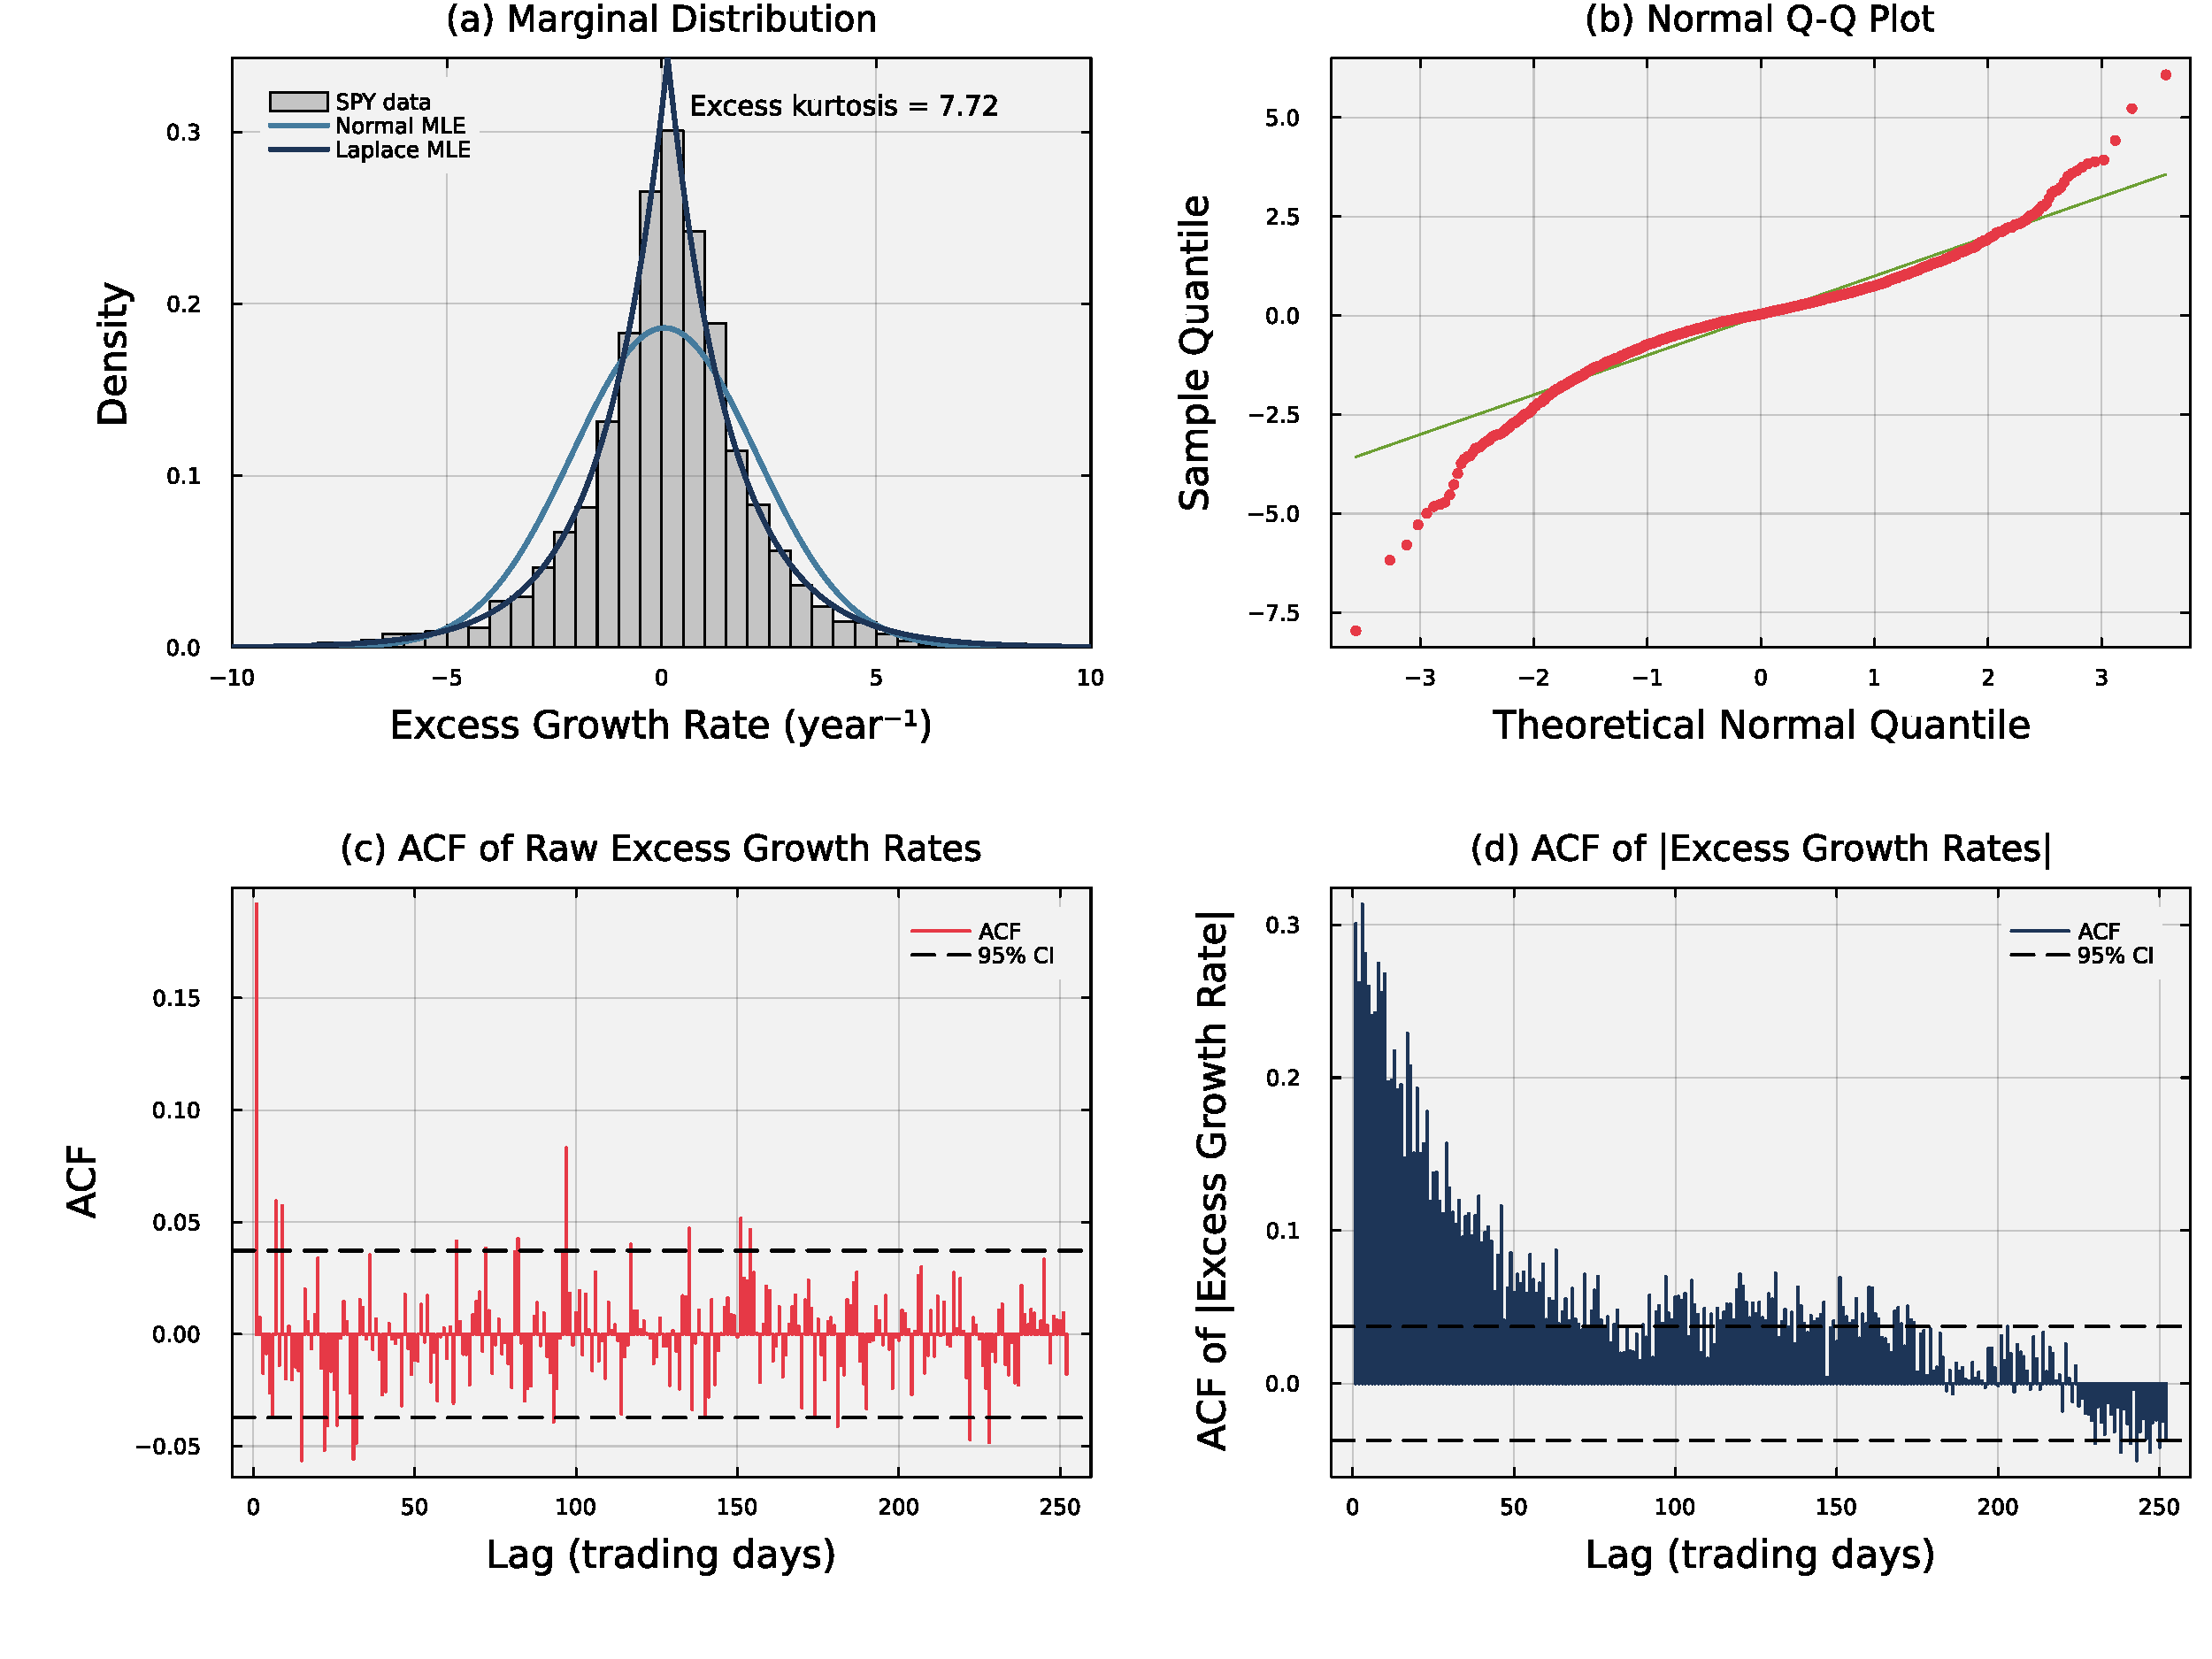
\includegraphics[width=\textwidth]{figs/main/Fig01-Empirical-Motivation.pdf}
    \caption{\textbf{Empirical stylized facts of SPY daily excess growth
    rates ($2014$--$2024$).} Panel~(a) shows the heavy-tailed return
    density; the Laplace maximum-likelihood fit tracks the empirical
    peak and tails while the Gaussian fit does not. Panel~(b) shows
    departure from the diagonal in a normal quantile-quantile plot
    at both extremes. Panel~(c) shows the
    autocorrelation function of raw excess growth rates. Individual
    correlations are small, although the Ljung--Box test detects joint
    serial dependence. Panel~(d) shows the autocorrelation function
    of absolute excess growth rates, which decays slowly across the
    reported lags.}
    \label{fig:empirical_motivation}
\end{figure}

\begin{figure}[H]
\centering
\resizebox{\textwidth}{!}{%
\begin{tikzpicture}[
  state/.style    = {circle, draw=black, very thick, minimum size=1.1cm,
                     inner sep=0pt, font=\small},
  tailbot/.style  = {state, fill=red!25,  draw=red!70!black},
  tailtop/.style  = {state, fill=blue!25, draw=blue!70!black},
  midstate/.style = {state, fill=white,   draw=black!70},
  markov/.style   = {<->, >=Stealth, thin, gray!80},
  trigger/.style  = {->, >=Stealth, thick, dashed, black!80},
  jumparc/.style  = {->, >=Stealth, very thick},
  note/.style     = {font=\footnotesize, fill=white, inner sep=2pt},
]
  \node[tailbot]              (s1)   at ( 0.0, 0) {$1$};
  \node[tailbot]              (s2)   at ( 2.0, 0) {$2$};
  \node[font=\Large]          (ld)   at ( 4.0, 0) {$\cdots$};
  \node[midstate]             (sk)   at ( 6.0, 0) {$k$};
  \node[font=\Large]          (rd)   at ( 8.0, 0) {$\cdots$};
  \node[tailtop]              (sNm1) at (10.0, 0) {$N\!-\!1$};
  \node[tailtop]              (sN)   at (12.0, 0) {$N$};
  \draw[markov] (s1)  -- (s2);
  \draw[markov] (s2)  -- (ld);
  \draw[markov] (ld)  -- (sk);
  \draw[markov] (sk)  -- (rd);
  \draw[markov] (rd)  -- (sNm1);
  \draw[markov] (sNm1)-- (sN);
  \draw[red!75!black, thick]
    plot[domain=-0.42:0.42, samples=40, smooth, variable=\t]
    ({ 0.0+\t}, {1.45 + 0.72*exp(-\t*\t/0.024)});
  \draw[red!25, thin] (-0.42,1.45) -- (0.42,1.45);
  \draw[red!75!black, thick]
    plot[domain=-0.42:0.42, samples=40, smooth, variable=\t]
    ({ 2.0+\t}, {1.45 + 0.72*exp(-\t*\t/0.024)});
  \draw[red!25, thin] (1.58,1.45) -- (2.42,1.45);
  \draw[black!55, thick]
    plot[domain=-0.42:0.42, samples=40, smooth, variable=\t]
    ({ 6.0+\t}, {1.45 + 0.72*exp(-\t*\t/0.024)});
  \draw[gray!40, thin] (5.58,1.45) -- (6.42,1.45);
  \draw[blue!75!black, thick]
    plot[domain=-0.42:0.42, samples=40, smooth, variable=\t]
    ({10.0+\t}, {1.45 + 0.72*exp(-\t*\t/0.024)});
  \draw[blue!25, thin] (9.58,1.45) -- (10.42,1.45);
  \draw[blue!75!black, thick]
    plot[domain=-0.42:0.42, samples=40, smooth, variable=\t]
    ({12.0+\t}, {1.45 + 0.72*exp(-\t*\t/0.024)});
  \draw[blue!25, thin] (11.58,1.45) -- (12.42,1.45);
  \node[draw, rounded corners=5pt, fill=yellow!20, very thick,
        minimum width=2.8cm, minimum height=1.1cm,
        align=center, font=\small] (clock) at (6.0, 5.0)
        {Poisson clock\\[1pt]prob.~$\epsilon$};
  \draw[trigger] (sk.north) -- (clock.south)
    node[note, midway, right=5pt, anchor=west] {jump triggered};
  \draw[jumparc, red!70!black]
    (clock.west)
    to[out=180, in=100]
    node[note, above, sloped, text=red!80!black,
         pos=0.45, yshift=3pt]
      {$K\!\sim\!\mathrm{Pois}(\lambda)$ forced steps}
    (s1.north);
  \draw[jumparc, blue!70!black]
    (clock.east)
    to[out=0, in=80]
    node[note, above, sloped, text=blue!80!black,
         pos=0.45, yshift=3pt]
      {$K\!\sim\!\mathrm{Pois}(\lambda)$ forced steps}
    (sN.north);
  \draw[decorate,
        decoration={brace, amplitude=6pt, mirror},
        red!70!black, thick]
    (-0.6, -0.65) -- (2.6, -0.65)
    node[midway, below=7pt, red!80!black, font=\small]
      {$\mathcal{S}_{-}$\ (bottom tail)};
  \draw[decorate,
        decoration={brace, amplitude=6pt, mirror},
        blue!70!black, thick]
    (9.4, -0.65) -- (12.6, -0.65)
    node[midway, below=7pt, blue!80!black, font=\small]
      {$\mathcal{S}_{+}$\ (top tail)};
  \draw[->, >=Stealth, gray!70, thin]
    (-1.0, -0.5) -- (13.2, -0.5)
    node[right, font=\small, text=black!70] {state index};
  \node[note, align=right, anchor=east, text=black!55]
    at (5.55, 2.72) {state emission\\[-1pt]
      $\mu_k\!+\!\sigma_k\cdot t_5$};
  \node[note, text=gray!80, anchor=west]
    at (6.55, 0.72)
    {prob.~$1\!-\!\epsilon$};
\end{tikzpicture}%
}
\caption{\textbf{Architecture of the hidden Markov model with jumps
    (HMM-WJ).} When no jump episode is active,
    the chain transitions according to the empirical transition matrix
    $\mathbf{T}$ with probability $1 - \epsilon$ (thin bidirectional
    arrows) or enters a Poisson jump episode with probability $\epsilon$
    (dashed upward arrow to the Poisson clock). During an episode, each of the
    $K \sim \mathrm{Poisson}(\lambda)$ forced steps independently draws
    the bottom tail set $\mathcal{S}_{-}$ (red, lowest-valued states)
    with probability $p_{\rm neg}$ or the top tail set $\mathcal{S}_{+}$
    (blue, highest-valued states) otherwise. Ordinary transitions then
    resume. Small bell curves above
    each state show the state-conditional location-scale Student-$t$
    ($\nu=5$) emission distribution. Tail sets are defined as the
    $N_{\rm tail}$ lowest- and highest-quantile states under the
    Laplace quantile partition.}
\label{fig:model_architecture}
\end{figure}

\begin{figure}[H]
  \centering
  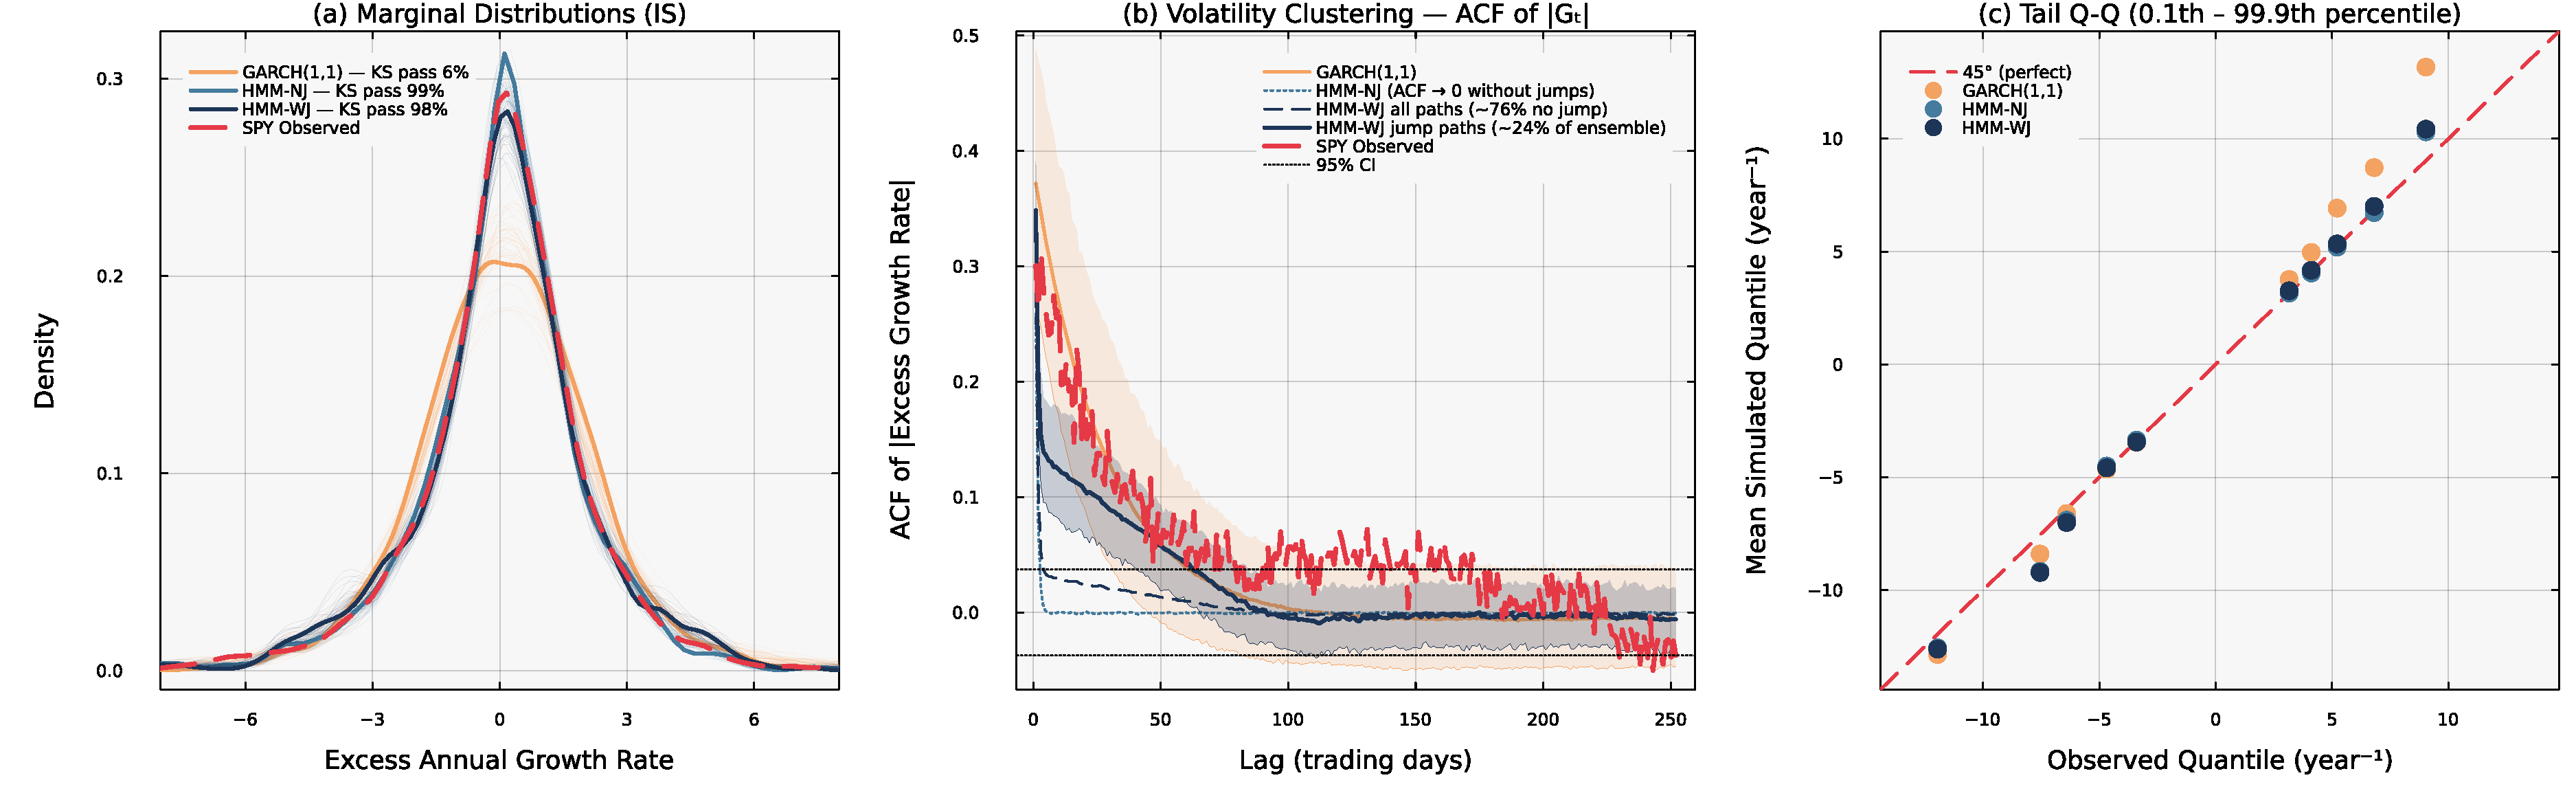
\includegraphics[width=\textwidth]{figs/main/Fig03-Model-Comparison.pdf}
  \caption{\textbf{Head-to-head in-sample model comparison for SPY}
    ($N = 100$, $1{,}000$ simulated paths). \emph{Panel (a):} marginal
    density of excess growth rates with in-sample Kolmogorov--Smirnov
    (KS) pass rates
    annotated per generator. \emph{Panel
    (b):} autocorrelation function of $|G_t|$ at lags $1$--$252$
    (shaded bands: $10$th--$90$th percentile across paths) per
    generator. \emph{Panel (c):}
    tail quantile-quantile plot at the $0.1$st--$99.9$th percentile region per
    generator.}
  \label{fig:model_comparison}
\end{figure}

\begin{figure}[H]
  \centering
  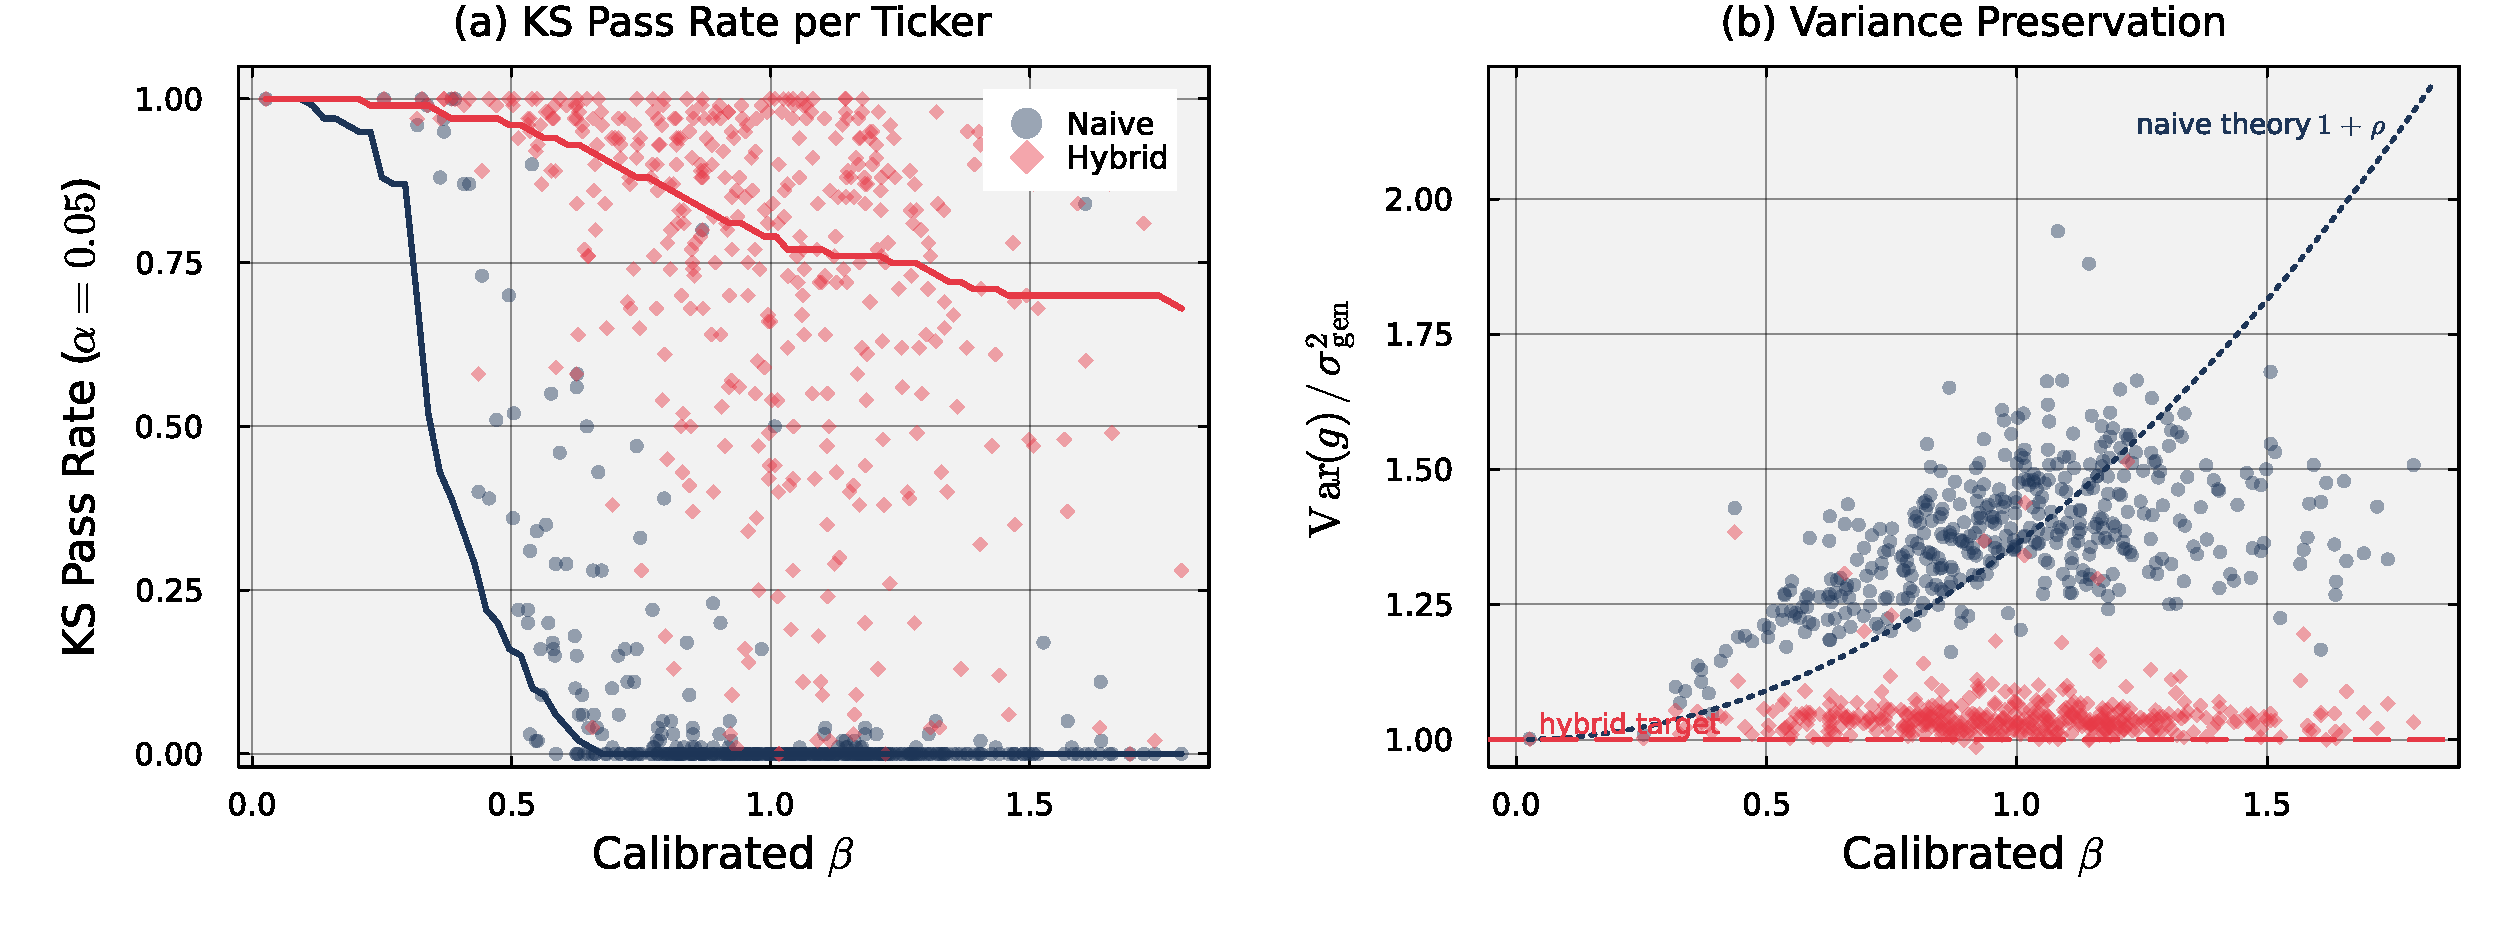
\includegraphics[width=\textwidth]{figs/main/Fig06-Variance-Preservation.pdf}
  \caption{\textbf{Effect of the hybrid variance correction on each
    ticker's Kolmogorov--Smirnov pass rate and variance ratio.}
    Each point is a per-ticker median over $100$ replications; thick
    lines are binned medians. \emph{Panel (a):} Kolmogorov--Smirnov
    pass rate against the real marginal at $\alpha = 0.05$ for naive
    composition (blue) and hybrid (orange).
    \emph{Panel (b):} variance ratio
    $\mathrm{Var}(g)/\sigma^2_{\mathrm{gen}}$ for the same two methods. The dotted curve is the
    theoretical naive inflation $1 + \rho$ evaluated at the universe-median
    $\sigma^2_{\mathrm{gen}}$ and the SPY annualized variance
    $\Delta t\,\sigma_m^2 = 0.030~\mathrm{yr}^{-1}$ of the closing-price
    series; the dashed line marks a variance ratio of one.}
  \label{fig:preservation}
\end{figure}

\begin{figure}[H]
  \centering
  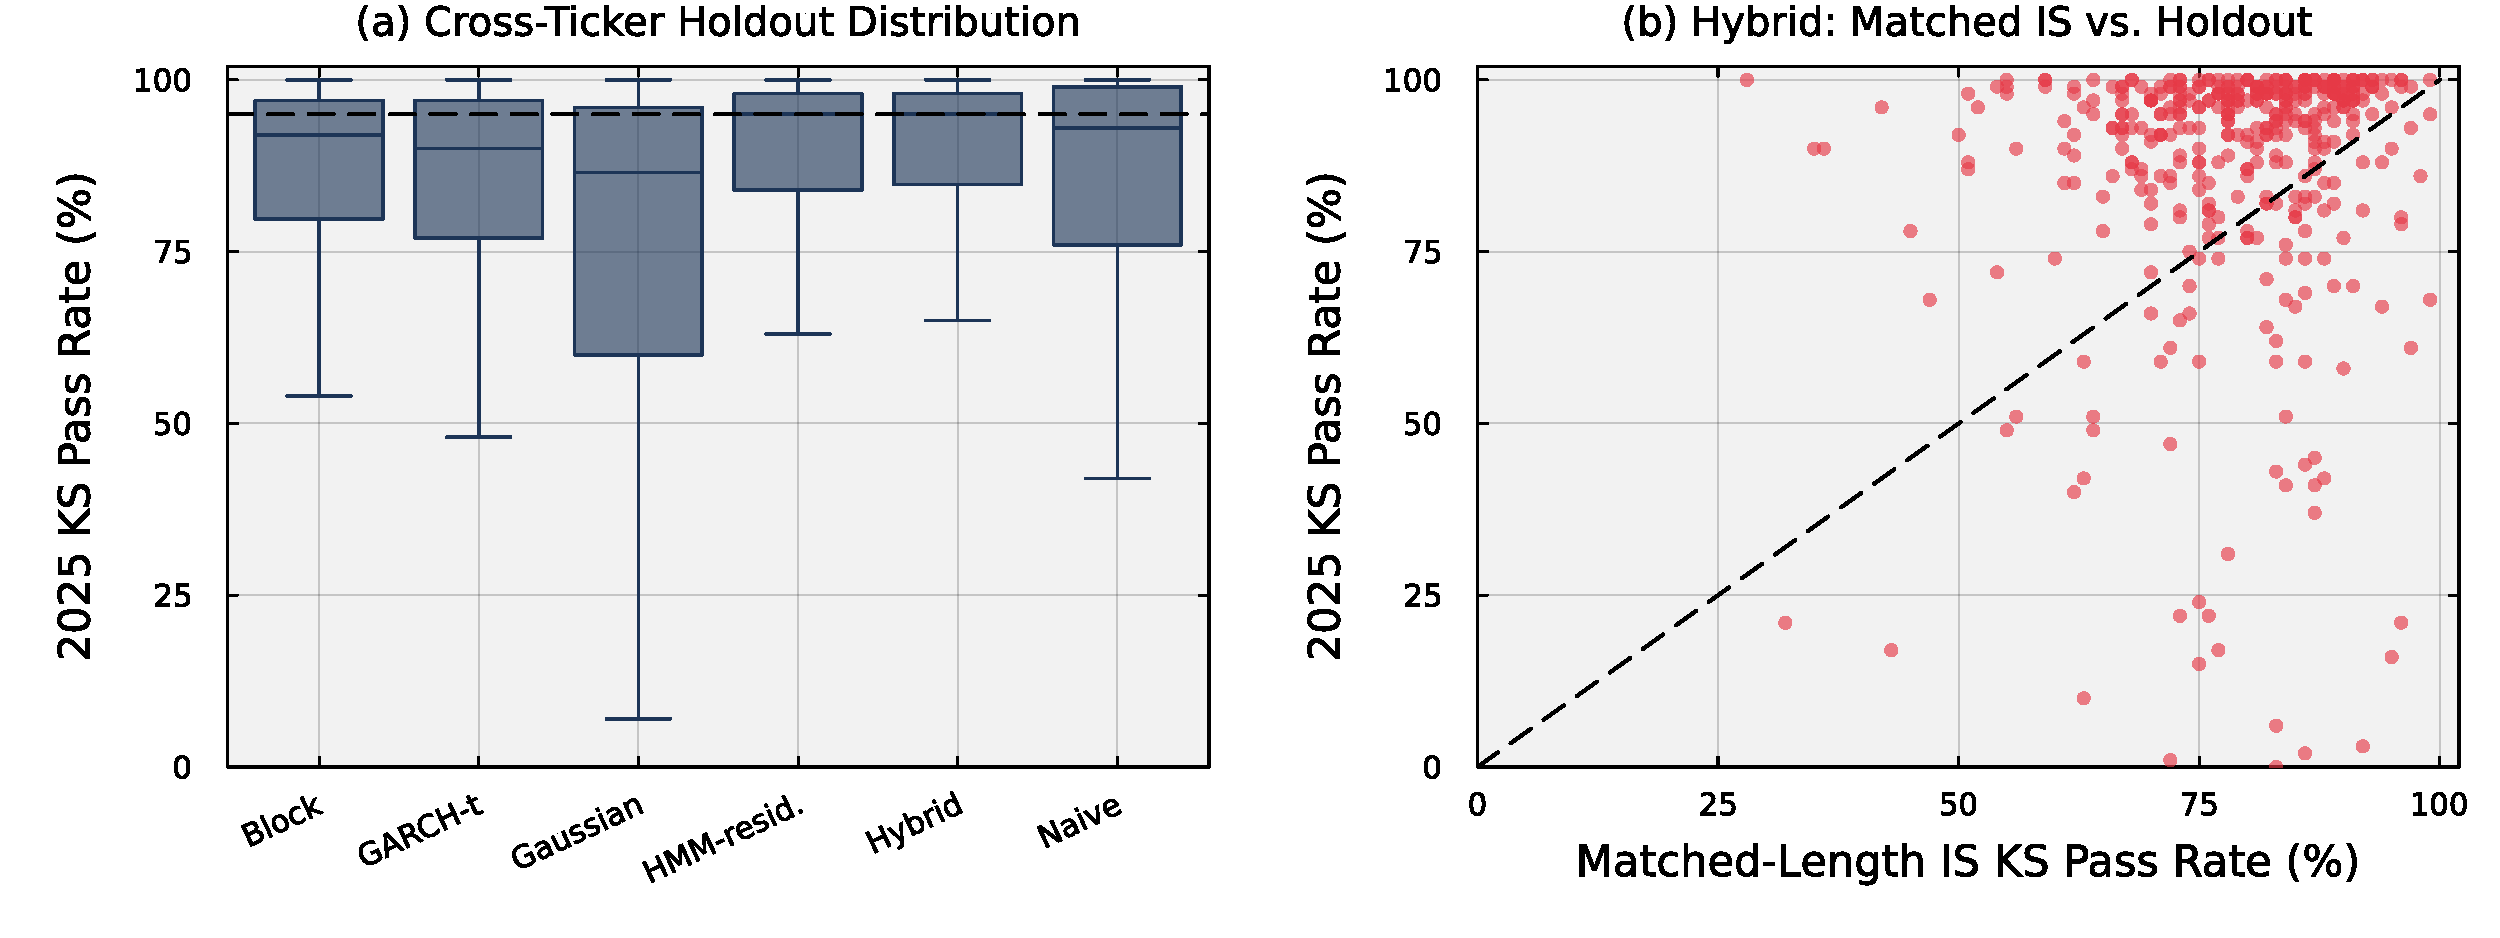
\includegraphics[width=\textwidth]{figs/main/Fig05-OoS-Composition.pdf}
  \caption{\textbf{Cross-ticker distribution of frozen-parameter
    out-of-sample marginal fit.} Panel~(a) shows the distribution of
    per-ticker $2025$ Kolmogorov--Smirnov (KS) pass rates across $100$ replications; the
    dashed line marks $95\%$. Panel~(b) compares each ticker's hybrid
    KS pass rate against a matched-length training block with its
    pass rate against the $2025$ holdout. The diagonal denotes equal
    performance.}
  \label{fig:oos_composition}
\end{figure}
